\documentclass[11pt]{article}
\usepackage[margin=1in]{geometry}
\usepackage{listings}
\usepackage{color}
\usepackage{epstopdf}
\usepackage{paralist}
\usepackage{graphicx}

\lstset{
    language=C++,
    basicstyle=\tiny,
    keywordstyle=\color{blue}\tiny,
    commentstyle=\color{magenta}\tiny,
    stringstyle=\color{red}\tiny
}

%% This is a comment
\begin{document}

\setlength{\baselineskip}{14pt}

\title{ECE408 Applied Parallel Programming Project: \\
       Checkers Board Game AI}

\maketitle

\newpage
\tableofcontents

\newpage
\section{Introduction}
English draughts (herein referred to as checkers) is a two-player zero-sum
perfect-information strategy game played on an 8x8 board. Opponents alternate
turns in which they move their pieces in an attempt to capture their opponent's
pieces.  The game is concluded when a player has no remaining pieces or can not
move any of their pieces.  In the event that the game is unlikely to conclude, a
tie is declared.

\subsection{Rules of Checkers}
For the purposes of this project, ``edge" cases in checkers are handled in the
following ways:

\begin{itemize}
  \item{The game is a draw after 100 plies.}
  \item{A player loses if they cannot make a move for any reason.}
  \item{Placing a piece in the row closest to your opponent turns the piece
into a king if it is not already.}
  \item{If a piece is kinged in the middle of a sequence of captures, the sequence is over.}
  \item{If a player has at least one available capture move, his move must be a capture move.}
\end{itemize}

Some board games include rules that repeated states or sequences of repeated
states cause the game to end in a draw. We use the rules above, where sequences
of repeated states are allowed. These are common tournament rules.

\newpage
\section{Problem Description}
In general, \textit{agents} (players) of zero-sum games with perfect
information are implemented on computers as a game-tree traversal.
Conceptually, the game tree is a directed tree where game states are the nodes
and edges between nodes describe the moves that transition between those game
states.

\begin{figure}[ht]
  \centering
    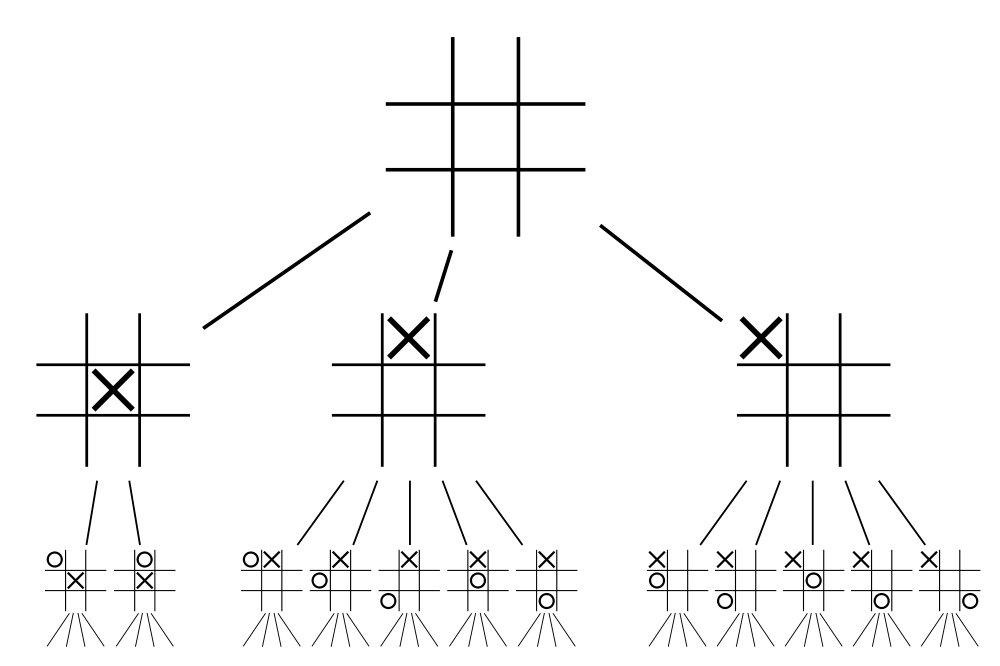
\includegraphics[width=0.7\textwidth]{pictures/gametree.png}
  \caption
  {
    Game tree\cite{gdr07} for the first two plys of Tic-Tac-Toe. Tic-Tac-Toe is
    a simple enough game that modern systems can quickly enumerate all
    possible game states.
    \label{fig:gametree}
  }
\end{figure}

Game trees can be characterized by about a half-dozen characteristics. There
are several that have a clear relationship with the game and do not require a
well-developed understanding of complexity. \textit{Board size} refers to the
size of the game board.
\textit{Average Game Length} is the average number of \textit{plies}, or
single-player moves, in a game. \textit{Branching Factor} is the average number
of game states that are produced from a particular game state. Table
\ref{tab:gametrees} shows these characteristics for a few common board games. 

\begin{table}[ht]
  \centering
  \begin{tabular}[ht]{ | r | c | c | c | }
    \hline
    Game & Board Size & Avg Game Length (plies) & Branching Factor\\ 
    \hline
    Chess    \cite{shannon50} & 64 & 80 &  35 \\
    Checkers \cite{allis94}   & 32 & 70 & 2.8 \\
    tic-tac-toe               &  9 &  9 &   4 \\
    connect4 \cite{allis94}   & 42 & 36 &   4 \\
    \hline
  \end{tabular}
  \caption
  {
    Game tree characteristics for common board games. 
    \label{tab:gametrees}
  }
  
\end{table}

These game trees are typically searched using the minimax algorithm or a
variant thereof. Conceptually, the procedure searches through the entire
game tree and only selects a move that would lead to an eventual victory. In
practice, game trees are too large to fully search. For
example, each level in a chess tree is $\approx$35 times larger than the one
before. By the time you look through one-quarter of the 80-ply length, there
are already 10\textsuperscript{25} nodes in the tree. This number can be
reduced by clever heuristics in the search, but it is still too large for the
entire tree to be enumerated.
To avoid this problem, the game tree is typically searched to a specific depth and
a heuristic score is applied to each terminal node. The value of each tree node
is then derived from the minimax algorithm of its children.

\newpage
\section{Implementation}

We developed two C++ CPU implementations, one hybrid C++/CUDA implementation and
one CUDA GPU implementation of a game-tree search for checkers. They are
described in the following subsections.

\subsection{CheckersBoard class \& TreeNode struct}

% TODO This section is kinda long. I first had it at one chunk of text, making
% it more compact but also harder to read. Should we remove some text? --Jesse

The CheckersBoard class and TreeNode struct are the most used data structures
across our different agent implementations. The CheckersBoard class is used by
all agent implementations presented in this work. The TreeNode struct is used by
both of the breadth-first agents.

The CheckersBoard class represents a checkers board, together with a number of
pieces and their locations. This class essentially contains a certain
game-state. The class contains numerous methods that assist in moving from one
game-state to the next. Some examples are: % methods
\begin{description}
    \item[\texttt{move(dst, src)}] Moves a piece from the source to the
    destination position on the board.
\item[\texttt{canMove(dst, src)}] Checks if a piece is located on the
    source location and can move to the destination position and.
\item[\texttt{p1NumPieces()}] Counts the number of pieces player 1 has.
\end{description}

% both on cpu as gpu
% 4 bytes

To make the implementation of CPU-GPU hybrid algorithms easier, we make the
CheckersBoard class usable by both the CPU and the GPU. This means the game tree
can be transferred onto and back from the GPU as-is.
We also pack the CheckersBoard data in the smallest possible package,
consisting of only three groups of four bytes, storing player one's pieces,
player two's pieces and the kings respectively. Using such a small data structure
enables us to transfer complete game-tree levels to and from the GPU in a small
amount of time.

The TreeNode struct is used by the breadth-first agents to build the game-tree, and
contains the following fields:

\begin{description}
    \item[\texttt{CheckersBoard board}] The state of the game.
    \item[\texttt{unsigned int parentIndex}] The array-index of its parent node.
        All
        parents are stores in the same array, so only its index is required to
        determine its position.
    \item[\texttt{int score}] The score or utility of the current game-state.
    \item[\texttt{bool hasChildren}] This value is true if there are other nodes
        that have their parentIndex point to this node.
\end{description}
\newpage
\subsection{CPU Breadth-First Search}
This section is not related to GPU programming, but the CUDA implementations
are direct parallelizations of these algorithms.
In some sense, CPU breadth-first search is the most straightforward evaluation
of the game tree. The search is seeded with a starting board and a number of
levels, and follows this algorithm.

\begin{lstlisting}
BFS(start, depth)
  
  for i in range(depth):
    generate next level

  evaluateLeaves(deepest level)

  for i in range(depth)
    propagate score up to previous level

\end{lstlisting}

First, the first \texttt{depth} levels in the tree are generated. The heuristic
is then applied to the boards in the deepest level, and then the scores from
each level are propagated up to the top of the tree. Finally, the child
of the starting board that has the best score is selected as the move. The
three distinct steps are described in the following sections.

Table \ref{tab:cpubfsprof} shows the most time-consuming portions of the CPU
BFS code. This information was used to inform the portions that we attempted
to accelerate using the GPU.

\begin{table}[ht]
  \centering
  \begin{tabular}[ht]{ | c | c | l | }
    \hline
    \% Time & Self Seconds & Name\\ 
    \hline
    25.23 & 245.43 & \texttt{evaluateLeaves()} \\
    15.20 & 147.92 & \texttt{possibleTakeoverMoves()} \\
    14.62 & 142.27 & \texttt{generate()} \\
    12.90 & 125.47 & \texttt{possibleSimpleMoves()} \\
     9.35 & 90.94  & \texttt{dequeue()} \\
     7.12 & 69.27  & \texttt{vector::insert} \\
    \hline
    100.0 & 973.16 & Total Execution Time \\
    \hline
  \end{tabular}
  \caption
  {
    Flat profile of CPU code. The first entry is the time spent evaluating
leaves. The next four entries are related to board generation. 
    \label{tab:cpubfsprof}
  }
\end{table}


\subsubsection{Board Generation: 50\% CPU Execution Time}
\label{sec:cpuboardgen}
The breadth-first board generation involves generating a child level made up of the children
of all the boards in the parent level.

\begin{lstlisting}
generteLevel(parentLevel)
  nextLevel = []
  for board in level:
    kids = children(board);
    add kids to nextLevel
  return nextLevel
\end{lstlisting}

To do this, we loop over each parent board and each game-board index in the
parent board.

\begin{lstlisting}
children(board, player1)
  captureChainBoards = []
  simpleMoveBoards = []
  for index in board:
    if index has player1 piece:
      captureChainBoards += captureChains(board, index)
      if [] == captureChainBoards:
        simpleMoveBoards += simpleMoves(board, index)
  if there are any moves:
    parent.hasChildren = true
  if [] == captureMoveBoards
    return simpleMoveBoards
  else
    return captureChainBoards
\end{lstlisting}

Since capture moves must be taken, we only generate the boards that result from
simple moves if there are no capture moves available. If there are capture
moves on the board, we return those, otherwise we return the simple moves. The
capture moves presented a challenge during board generation since multiple
capture jumps can be made in a single ply in the tree. See Section 
\ref{sec:generalchallenges} for more details.

\subsubsection{Leaf Evaluation \& Scoring Heuristic: 25\% CPU Execution Time}
When the last level of the tree is generated, each board must be scored so that
the score propagation step can generate scores for the parents of those boards.
\begin{lstlisting}
evaluateLeaves(level)
  for board in level:
    utility(board)
\end{lstlisting}
Our CPU code sequentially applies a scoring heuristic to each board in the last
level. A positive score indicates the board favors Player 1, and a negative
score indicates the board favors Player 2. A zero indicates the board is even.

\begin{lstlisting}
utility(board):
  if player1 wins: return INT_MAX
  if player2 wins: return -INT_MAX
  if tie:          return 0

  p1score = board.p1WeightedMen()
  p2score = board.p2WeightedMen()

  if (p1score > p2score)      return  p1score / p2score * MULTIPLIER;
  else if (p1score < p2score) return -p2score / p1score * MULTIPLIER;
  else                        return  0

\end{lstlisting}
The scoring heuristic generates an integer score for each board. If Player 1 is
the victor in the board, it returns INT\_MAX. If Player 2 is the victor, it
returns -INT\_MAX. If the board results in a tie, it returns 0. Otherwise, it
generates a weighted sum of the pieces that each
player has. The pieces are weighted by how far they have advanced along the
board, and a king piece has a static weight higher than that of the most
valuable man regardless of the king's position. Dividing the weighted values
allows the player with the advantage to favor trading pieces. 
\texttt{MULTIPLIER} is a value used to spread the fractional division result
evenly across the whole integer space.


\subsubsection{Score Propagation: $<$5\% CPU execution time}
\label{cpupropagation}
After the leaves are scored, each parent board should end up with the score of
its best child. The meaning of "best" is dependent on whether the children
were generated by Player 1 or Player 2 moving. If Player 1 moved, the best child
has the highest score, and if Player 2 moved, the best child is the lowest
score.

\begin{lstlisting}
propogateScore(parentLevel, childLevel, player1)
  for board in childLevel:
    parentIndex = board.parent
    parentScore = parentlLevel[parentIndex].score
    if player1:
      if child.score > parentScore:
        parent.score = child.score
    else if child.score < parentScore:
        parentLevel[parentIndex].score = child.score
\end{lstlisting}

At each level, the children are all inspected. A child board knows in the index
of its parent, so it is simple to compare the child score with the parent
and update the parent if the child has a better score than has so far been
found. This is done for each level starting at the largest, until every board
in the tree has a score. This is less than 5\% of the total execution time.
\newpage
\subsection{Hybrid Breadth-First Search}
The hybrid breadth-first search is exactly the same as the pure-CPU
breadth-first search, but with certain operations accelerated on the GPU.
Sections \ref{sec:GPUboardgen}, \ref{sec:GPUleafeval}, and 
\ref{sec:GPUscoreprop} describe the three accelerated operations.

\subsubsection{Board Generation}
\label{sec:GPUboardgen}
Board generation takes about 40\% of the sequential execution time, and
therefore is a good candidate for acceleration on the GPU. The downside is that
small differences in board layout can lead to large changes is code execution.

In an effort to keep the implementation as simple as possible, each parent
board was assigned to a single thread that would be responsible for generating
all of the children of that board. Other options include assigning one thread
to each child board, or assigning one thread to each piece or index in the 
parent board. Those options were all rejected because it would involve most
threads not doing any work: for most of the game less than half of the board
is occupied, and a board can have an extremely variable number of children. In
the smallest case, only a single capture move may be
available, and in more complicated cases around 10 pieces may be able to move
into six or eight squares. 

All boards in the parent level are copied
into GPU global memory, and GPU global memory that is guaranteed to be larger
than the number of child boards is also allocated. The GPU fills the child
board array with child boards, and also reports the number of child boards
it generated so the CPU knows how many to copy back.

\begin{lstlisting}
GPUBoardGeneration(parentBoards):
  maxNumChildBoards = numChildBoards(parentBoards)

  cudaMalloc(maxNumChildBoards)
  cudaMalloc(numParentBoards)
  cudaMalloc(unsigned numGeneratedChildBoards)

  cudaMemCpy(device parentBoards <- host parentBoards, numParentBoards)
  
  launch kernel

  cudaMemCpy(host numGeneratedChildBoards <- device numGeneratedChildBoards, 1)
  cudaMemCpy(host childBoards <- deviceCHildBoards, numGeneratedChildBoards)
  cudaMemCpy(host parentBoards <- device parentBoards, numParentBoards)
\end{lstlisting}

This means that the potential parallelism
is low early in the game tree where there are not very many boards. The idea is
to do the early evaluations on the CPU and once the levels get large enough,
move them to the GPU. Conceptually this is quite simple, and works well, but
there were a number of difficulties in the transition that are described in
Section \ref{sec:hybridbfschallenges}.



\subsubsection{Leaf Evaluation}
\label{sec:GPUleafeval}
Leaf evaluation is an embarrassingly parallel problem and a significant chunk
of the CPU execution time. We implemented a GPU kernel that assigns a single
thread to each board in the leaf level and applies the utility heuristic to it.
This approach was very simple and successful. Our results can be found in
Section \ref{sec:bfsresults}.


\subsubsection{Score Propagation}
\label{sec:GPUscoreprop}

Although we have seen that the score propagation is responsible for less than
5\% of the execution time, the problem is still
embarrassingly parallel and could profit from parallel execution. Similar to the
CPU implementation described in Section \ref{cpupropagation}, we want to
propagate the maximum score if we are player 1, and the minimum score if we are
player 2.

The treenode objects we use to build our tree are aware of the index of their
parent node, but not of their children nodes. Because we do not want to search
for treenodes in our kernel, we assign each thread to a treenode in the lower
level. This enables threads to directly access the parent of its assigned
treenode, by using the parentIndex pointer in the treenode struct. Because each
thread compares the score of its assigned node with the parent node, and
treenodes are likely to have multiple children, atomic operations are required
when we propagate the scores in parallel.

\begin{figure}
\begin{lstlisting}
  if(id < lowerSize)
  {
    treenode* parent = &upperLevel[mynode.parentIndex];
    bool didSwap = false;
    while(!didSwap)
    {
      int parentScore = parent->score;
      // If we are player one and our score is smaller than the current score in
      // the parent, break. We are trying to maximize.
      if(p1 && mynode.score <= parentScore) break;
      // If we are player two and our score is greater than the current score in
      // the parent, break. We are trying to minimize.
      if(!p1 && mynode.score >= parentScore) break;
      int old = atomicCAS(&(parent->score),parentScore, mynode.score);
      if(old == parentScore)
      {
        didSwap = true;
      }
    }
  }
\end{lstlisting}
\caption{A code snipper from the score-propagation kernel that compares and
writes scores to its parent using atomics.}
\end{figure}

\newpage
\subsection{Depth-First Search}
\label{sec:gpudfs}

The Depth-First Search algorithm, unlike the Breadth-First Search, focuses on
analysing future plies before analysing alternatives of the current ply. This
gives it a distinct advantage over the breadth-first search when it comes to
memory usage. As an example, a serial breadth-first search of checkers to depth
10 should require the storage of about 2.8\textsuperscript{10} = 29620 game
states, where a depth-first search would only need to maintain 10 game states.

\subsubsection{CPU Depth-First Search}

As a reference model for our GPU-based depth-first search implementation, we
first build a CPU-based game agent. This game agent allows us to quantify the
results we obtain from our GPU-based game agent.

Our CPU depth-first search agent is a basic Minimax game agent. The agent is
single-threaded and uses Alpha-beta pruning to improve performance. It
is the text-book example of a standard game agent.

This implementation does not use any ordering heuristic when evaluating leaves.
Different heuristics can be tried to further improve the effectiveness of
Alpha-beta pruning, but this is not in the scope of this work.

\subsubsection{GPU Depth-First Search}
\label{sec:GPUDFSalgo}

Taking advantage of the reduced memory footprint of depth-first search, the
entirety of minimax can be run on the GPU, minimizing CPU-GPU communication
delays. To start the algorithm, the CPU must copy to the GPU a board that it
wishes to determine the best subsequent board of. This board is then copied from
global memory to the beginning of a shared memory stack.  All preceding
operations occur in shared memory.

In an effort to maximize parallelism and minimize wasted calculations, the GPU's
depth-first search then generates all of the child boards(1 ply deep) in
parallel of the given parent board and saves them to a stack. Taking advantage
of the GPU, the tiles on the checker board are each assigned to one of 32
threads in the block(1 warp size). This allows the generation function to
immediately find the tiles with moveable pieces, and eliminates one of the loops
necessary in the CPU implementation. Following generation of a child board, the
board is turned. This simplifies the code and reduces the number of branches
necessary as the algorithm is able to play as if its player 1 at all times.
Finally a stackPointer is atomicly incremented allocating space for the new
boards in the stack, and the boards are saved. 

\begin{lstlisting}
pseudo code high level overview of board generation from a child
void genChildren(CheckersBoard* boardStack, int* boardStackPointer, CheckersBoard boardToExpand)
{
    //square that this thread deals with
    unsigned int squareIndex = ((threadIdx.x%32) + 1)*2-1 - (threadIdx.x/4)%2;  
    //there are 8 possible moves, 4 directions times 2 types of moves {attack,nonattack}
    for each moveToCheck = movePossible
    {
        if(boardToExpand.canMove(squareIndex, moveToCheck))
        {
            CheckersBoard newBoard = boardToExpand;
            newBoard.move(squareIndex, moveToCheck);
            newBoard.rotate();
            int indexToSaveTo = atomicAdd(boardStackPointer, 1);
            boardStack[indexToSaveTo] = newBoard;
        }
    }
}
\end{lstlisting}

Following the generation of potential child boards, a single board is picked
from the sub stack of newly generated boards, and the process repeats generating
one deeper plies worth of boards. This process continues to repeat until the
deepest ply desired is reached.

\begin{lstlisting}
pseudo code generate boards till maxDepth
void genBoardsToMaxDepth(CheckersBoard* boardStack,
        int* boardStackPointer,
        int maxDepth)
{
    while(ply<maxDepth)
    {
        //all threads pick the same boardToExpand
        CheckersBoard boardToExpand = pickBoardToExpand(boardStack,
            *boardStackPointer); 
        genChildren(boardStack, boardStackPointer, boardToExpand);
        ply++;
    }
}
\end{lstlisting}

Once the deepest ply has been reached, the heuristic function is applied in
parallel to the deepest boards. Then a parallel reduction operation is used to
determine the highest scoring board. This score is then negated, and saved as
the score of the board's parent. The reason for this negation is the use of the
negamax simplification. This simplification takes advantage of the zero-sum
nature of checkers, essentially assuming that player 1's utility of a given game
state is the negative of the utility of player 2 in that game state. This
simplification, allows the minimax algorithm to always search for the maximum
heuristic score, instead of having to maximize half the plies and minimize the
other half.

\begin{lstlisting}
pseudo code scoring and sorting
void getBestScore(int parentBoardIndex,
        CheckersBoard* boardStack,
        int beginingOfBoardsToScore,
        int endOfBoardsToScore,
        int* bestScore,
        float* placeToKeepTrackOfScores)
{
    
    for(int i = beginingOfBoardsToScore + threadIdx.x; i < endOfBoardsToScore;
            i+=blockDim.x)
    {
        //each thread helps score
        placeToKeepTrackOfScores[i] = heuristic(boardStack[i]);
    }
    //threads work together to find the max and put it in the first index
    findMaxWithReduction(placeToKeepTrackOfScores, beginingOfBoardsToScore,
            endOfBoardsToScore);
    //the score is negated due to negamax
    placeToKeepTrackOfScores[parentBoardIndex] = - placeToKeepTrackOfScores[beginingOfBoardsToScore];
}
\end{lstlisting}

After scoring of the final ply is complete, the final plies stack is cleared by
resetting its sub stack pointer. Then the parent's ply is checked to determine
what boards remain to be expanded from that ply. If there are no boards
remaining to be expanded, the reduction operation is applied and the highest
score for this ply is negated and propagated to its parent. Then the lowest
sub-stack is cleared, and the process repeats propagating scores to higher
levels until an unexpanded board is discovered. Once an unexpanded board is found
the process repeats, starting with the generation of boards.  Finally, all of
the immediate successor boards of the first board provided by the CPU are scored
and the best one is returned to the CPU.

\subsubsection{Issues with Pure Depth-First Search on the GPU}
\label{sec:GPUDFSissues}

As a result of depth-first search's substantially reduced memory footprint, the entirety of the
depth-first search can be run on the GPU. This means that communication delays
between the CPU and GPU are substantially less than that of the breadth-first
GPU implementation. While these benefits in theory should make the depth-first
minimax a superior algorithm to run on the GPU vs the breadth-first search, our
experiments suggest otherwise.

One of the primary reason's our GPU only depth-first minimax search proved to be
the poorest performer of all of the implementations tested was the significantly
limited parallelism available to a pure depth-first approach. This meant that
while board generation was a parallel operation, it was not parallel enough to overcome
the GPU's slower clock rate when compared to a CPU.

\subsubsection{Improving Depth-First Parallelism with Breadth-First CPU into Depth-First GPU Hybrid}
\label{sec:GPUDFSimproved}

One way of improving parallelism on the GPU is to use more blocks. In our first implementation of
depth-first search, we only provided the GPU with one board to work with. By combining our breadth-first
search CPU implementation with the depth-first GPU implementation we were able to achieve huge increases
in performance over the pure depth-first GPU version, actually beating the CPU only version on deep searches.
To do this, we provide our breadth-first CPU implementation a starting board and used it to generate a few
plies deep. Then we use the lowest ply generated, as input to the GPU's depth-first implementation. 
Each board at the lowest level of the breadth-first CPU is assigned
to a block on the GPU. This allows the GPU to mask memory lag, and branch evaluation costs by switching between
blocks as it searches. Eventually the GPU depth-first code completes providing the scores of the last boards of the
CPU breadth-first search. These scores are then propagated through the breadth-first tree, eventually producing a
minimax solution.

\newpage
\section{Results}
\subsection{Hybrid Breadth-First Search \& CPU Breadth-First Search Results}
\label{sec:bfsresults}


\begin{table}[ht]
  \centering
  \begin{tabular}[ht]{ | c | c | }
    \hline
    Parent Level Size & Speedup \\ 
    \hline
    2      & 0.0125 \\
    6      & 0.0436 \\
    42     & 0.1366 \\
    170    & 0.8284 \\
    994    & 0.9062 \\
    3823   & 1.7197 \\
    19530  & 1.5611 \\
    73011  & 2.3971 \\
    355722 & 1.5428 \\ 
    \hline
  \end{tabular}
  \caption
  { 
    GPU Board Generation Speedup vs Input Size 
    \label{tab:bfsboardgenspeed-up}
  }
\end{table}

\begin{table}[ht]
  \centering
  \begin{tabular}[ht]{ | c | c | }
    \hline
    Leaf Level Size & Speedup \\ 
    \hline
    2      & 0.0292 \\
    6      & 0.0619 \\
    42     & 0.3462 \\
    170    & 1.3650 \\
    994    & 6.7041 \\
    3823   & 18.683 \\
    19530  & 29.654 \\
    73011  & 35.653 \\
    355722 & 28.220 \\ 
    \hline
  \end{tabular}
  \caption
  {
    GPU Leaf Evaluation Speedup vs Input Size
    \label{tab:bfsleafevalspeed-up}
  }
\end{table}

\begin{figure}[ht]
  \centering
    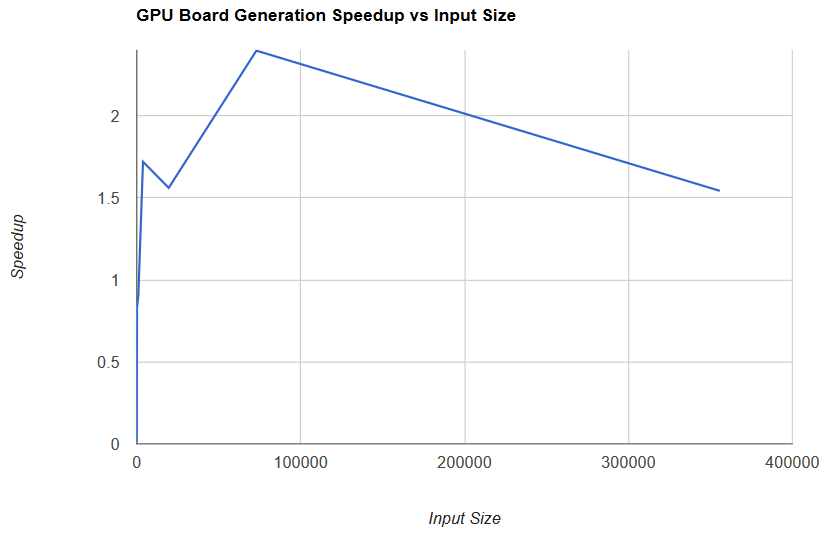
\includegraphics[width=0.5\textwidth]{pictures/bfs_board_gen_speedup.png}
  \caption
  {
    Speed-up of GPU board generation for various parent level sizes.
    \label{fig:bfsboardgenspeed-up}
  }

\end{figure}


\begin{figure}[ht]
  \centering
    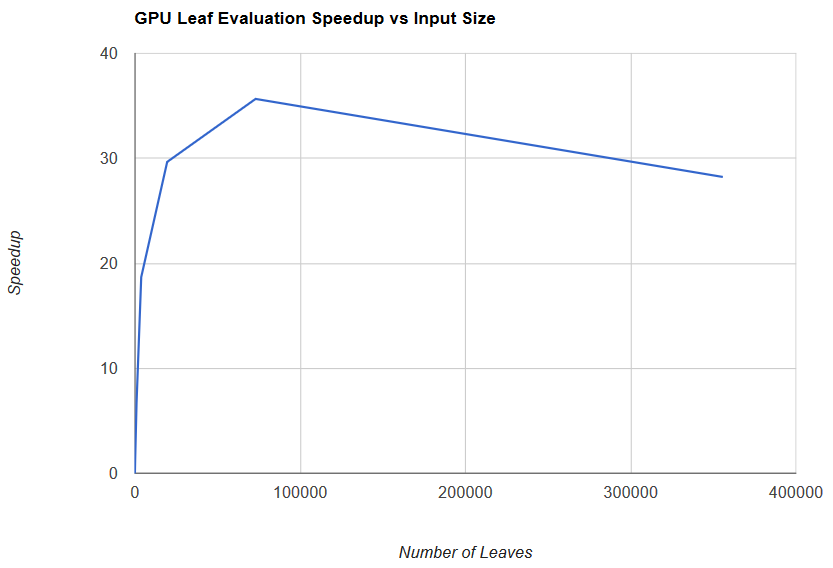
\includegraphics[width=0.5\textwidth]{pictures/bfs_leaf_eval_speedup.png}
  \caption
  {
    Speed-up of GPU leaf evaluation for various leaf level sizes.
    \label{fig:bfsleafevalspeed-up}
  }
\end{figure}

In summary, accelerating board generation by 1.5x and leaf evaluation by 30x
should yield a 1.7x speed-up in total breadth-first board evaluation. The speed-up from 
score propagation is significant, but it's percentage of CPU run time prevents
it from impacting the results.

\newpage
\subsection{GPU \& CPU Depth-First Search \& Hybrid Breadth-First/Depth-First Search Results}

Unlike the breadth-first algorithms, the depth-first algorithms do not generate entire levels
of the game tree explicitly. Instead, levels are both
generated and evaluated piece by piece while the algorithm is exploring
different branches. Because of this, timing these individual steps becomes more
difficult. To compare our CPU, GPU, and Hybrid implementations, we had the algorithms
play complete games of 100 turns. We then varied the search-depth and recorded the total game runtime.

\begin{figure}[!ht]
    \begin{center}
        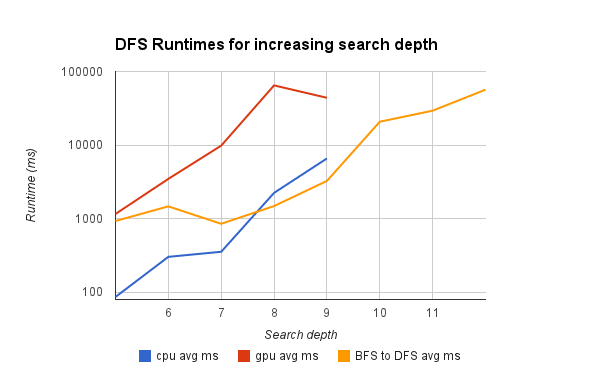
\includegraphics[width=0.8\textwidth]{pictures/gpu_cpu_dfs_runtimes.png}
        \caption{Runtime of GPU and CPU Pure Depth-First Search and Hybrid agents.}
        \label{fig:gpucpudfsruntimes}
    \end{center}
\end{figure}

As can be seen in Figure \ref{fig:gpucpudfsruntimes}, the CPU depth-first search performed about 10x better than the pure GPU implementation on board counts 5 - 9.
After depth 9 the pure GPU implementation would run out of time on the GEM cluster, and the process would be killed. These results contrast sharply with the
breadth-first to depth-first hybrid tests. In these tests we see the initially high cost of GPU code when the problem size is not big enough, and then we observed the hybrid code
actually out preforming the CPU only implementation for search depth 8 and greater. At these depths, there were thousands of blocks available to the GPU,
promoting efficient block scheduling and improving performance.
    Unfortunately, due to differences in implementation and tie breaking
strategies of our CPU, GPU, and Hybrid versions, the game play between versions varied considerably. This resulted
in games of different lengths being played by the two versions of the code, skewing results. Another interesting
limitation of this benchmarking strategy was the effect of different board layouts on runtime. Specifically, boards
that had few moves available, took less time to evaluate(as they should).

\newpage
\section{Challenges}

\subsection{General Challenges in Checkers Game-Tree Search}
\label{sec:generalchallenges}
The most difficult part of the checkers tree search is the combination of a
series of capture moves into a single edge in the tree. This description is not
specifically related to CPU programming, but the GPU is required to emulate the
same functionality in its implementation.

The way all of our CPU implementations solve this is by creating a queue of
boards and piece indexes. When a capture move is discovered, the resulting
board and index of the piece that made the capture move is added to the queue.
As long as the queue isn't empty, we remove a board/piece combination and
inspect that piece on that board to see if more capture moves are available. If
they are, the resulting board/peice combinations are added to the queue. If 
there are none, the board is a terminal board from a chain of capture moves,
and qualifies as a child board of the initial board.

\subsection{Challenges in Hybrid Breadth-First Search}
\label{sec:hybridbfschallenges}
Since we used one thread for each parent board in board generation, the only
significant difficulty in transitioning to CUDA code was that the
dynamically-growable data structures used in the CPU code had to be mapped into
static arrays on the GPU. These dynamic data structures were used in the CPU
because the only way to tell how many children a particular board will have is
to generate them all and count them. Doing a pass to determine the number of
generated boards and then a second pass to generate them would roughly double
the amount of computation necessary for board generation.  Furthermore, it is
impossible for a GPU kernel to dynamically allocate memory to itself. This means
that the following dynamic CPU data structures had to be remapped into static
structures on the GPU

\begin{itemize}
  \item{Queues used to investigate takeover chains}
  \item{Lists to accumulate the simple moves available to a piece}
  \item{Lists to accumulate the simple moves available to a board}
  \item{Lists of takeover moves}
\end{itemize}

Based on the description in Section \ref{sec:cpuboardgen}, a queue is not
strictly required. We replaced the queues in the breadth-first CPU board generation code
with stacks in the GPU. A stack is just an array and a variable to point at the
top, and a list is just an array with a variable to point at the end. Those two
objects look exactly the same when they are implemented using a static array
and an indexing variable.

These static arrays are kept in shared memory, and each thread needs its own.
Since those arrays have to be big enough to handle the worst-case size of the 
list and stack, each thread ended up requiring a significant amount of memory.
In our CUDA code, the arrays were defined this way:

\begin{lstlisting}
#define GENERATE_BLOCK_SIZE 12
const unsigned PSMR_SIZE = 4;
const unsigned PCCR_SIZE = 8;
const unsigned TEST_SIZE = 12;
const unsigned SMR_SIZE = PSMR_SIZE * 12;

  __shared__ CheckersBoard pieceSimpleMoveResults[GENERATE_BLOCK_SIZE][PSMR_SIZE];
  __shared__ CheckersBoard simpleMoveResults[GENERATE_BLOCK_SIZE][SMR_SIZE];
  __shared__ CheckersBoard pieceCaptureChainResults[GENERATE_BLOCK_SIZE][PCCR_SIZE];
  __shared__ CheckersBoard testBoardStack[GENERATE_BLOCK_SIZE][TEST_SIZE];
  __shared__ unsigned char testIndexStack[GENERATE_BLOCK_SIZE][TEST_SIZE];
\end{lstlisting}

A CheckersBoard is 13 bytes, so each thread needs roughly a kilobyte of shared
memory if there is zero padding in any of the arrays of structures. In practice,
we are limited to 12 threads per block, and only one block running on an SM at
a time. This is an enormous reduction on the possible parallelism potential of
board generation.

There is also a massive amount of control divergence in the board generation
code. This partially a result of the divergent nature of board game states, and
partially a result of the choice to use one thread for each parent board. Some
opportunities for control divergence to occur in the code are listed below:

\begin{itemize}
  \item{A board index is occupied}
  \item{The piece is a king or a man}
  \item{The piece belongs to player 1 or player 2}
  \item{the 2-4 spaces the piece can move to are in various states of occupation}
  \item{the 2-4 spaces the piece can capture are occupied or not}
  \item{Capture moves are or are not available}
\end{itemize}

Some of these can be mitigated by assigning one thread per board index instead
of one thread per board, but then those threads must coordinate their work,
which increases the code complexity.

\subsection{Challenges in Depth-First Search}
As previously noted, the greatest challenge of writing a depth-first search to run on the GPU is finding enough parallelism.
As a result of the GPU's need for parallelism, pure depth-first search is not a good algorithm to attempt on a GPU as it is inherently serial.
To promote parallelism within our GPU implementation, we decided to generate several boards at once, instead of the single board at a time approach dictated by traditional depth-first search.
This meant that we were not able to use a simple stack to maintain information about previous game states visited. Instead we had to keep several stacks, one for each level of search
we were going to preform. 

\begin{figure}[!ht]
    \begin{center}
        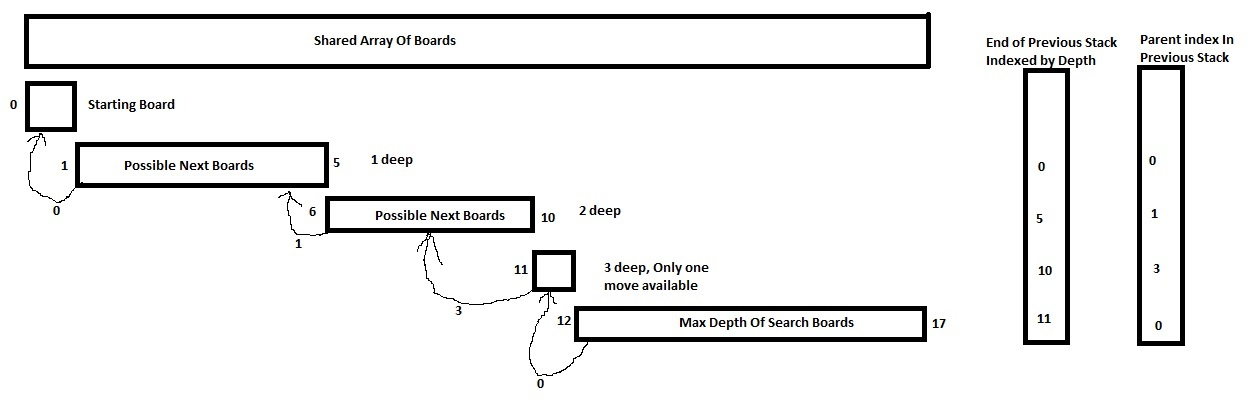
\includegraphics[width=1\textwidth]{pictures/Picture_of_Stack.jpg}
        \caption{Shared Stack with Sub-Stacks}
        \label{fig:stackPicture}
    \end{center}
\end{figure}

    To minimize memory consumption, we decided to not allocate each of these sub stacks individually. Instead we used a single shared memory array that was sized to be able to contain
the worst-case sum of all the sub stacks we were going to generate. To keep track of each of these stacks, a separate shared array was allocated containing pointers to the end of each sub stack.
Finally, a third array of counters was allocated, representing the stack pointers of each respective sub stack. As a result of this set up, multiple boards could be generated at once, and all scoring
propagation could be done with the use of parallel reduction. While these benefits were necessary for a GPU implementation, the complex stack operations complicated the code
significantly. See figure \ref{fig:stackPicture} for a graphical explanation.
    
    After implementing the depth-first search on GPU, connecting it to the breadth-first CPU search
presented some difficulty. Namely, the CPU code took advantage of the CPU's ability to branch frequently
this resulted in code that did not assume it was player 1 all the time as the GPU code did. To fix this
a conversion of the boards generated by the CPU had to be applied before they boards were ready to be used on the GPU.
After the GPU had finished its analysis, the hybrid code then had to convert the scores on the boards into
the appropriate sign so that the CPU breadth first would analyse them correctly.


\newpage
\section{Future Work}
\subsection{Future Work in Pure GPU Depth-First Search}
While the depth-first search seems well suited to the memory limitation of the GPU, its limited parallelisms limits its effectiveness. Due to this
observation, I would not recommend anyone attempt to run a purely depth-first approach on the GPU. Instead, I would expect that great gains in search could be derived from
a combined approach utilizing a wider, pseudo depth-first and breadth-first hybrid.
\subsection{Future Work in Hybrid Depth-First Search}
While our experiments demonstrated the limited parallelism of pure depth-first search, our breadth-first experiments proved that the GPU can be used to enhance search speed.
I believe that by combining the two searches,(namely by searching multiple branches of the tree at once, while only maintaining a small portion of the tree) a superior
GPU search algorithm will be discovered.
\subsection{Future Work in Hybrid Breadth-First Search}
Reducing the amount of shared memory in each thread would increase the pressure
on the global memory system, but would also allow more parallelism which could
mask that pressure. Future work would be to move all of the shared arrays into
global memory, which would vastly increase the number of threads per block.

\section{Conclusion}

% General conclusion

We have implemented two different GPU-based checkers game-agents. One using
breadth-first search, and one using depth-first search. 
% BFS Results
In the breadth-first implementation, we see significant speed-up in multiple
areas compared to the CPU version.
% Speedup in leaf evaluation
We obtain a ~30X speed-up in the leaf evaluation of the breadth-first search
agent when we perform this operation on the GPU. The leaf evaluation accounts
for more than 25\% of the total execution time on the CPU, which causes the
speed-up to have a significant impact on the total runtime.
% Speedup in board generation
We also obtain a ~1.5X speed-up in the generation of new boards for the
breadth-first search agent. The generation of boards accounts for 50\% of
the total execution time on the CPU, but the limited improvement in that 
section has only a small effect on the total runtime. Through a different
trade-off between shared memory usage and block size, this result may be
able to be improved.

% DFS Results
In the depth-first implementation, we observed a significant decrease in performance
when we move our implementation to the GPU. 
% Lack of improvement, due to lack of parallalism
This decrease in performance is most likely due to the lack of parallelism available when evaluating only a single branch of the game tree at a time. To counteract these limitations,
our hybrid version, used breadth-first CPU code to first expand the initial board. Then the leafs of the breadth-first search were used as the initial boards of the GPU depth-first search.
This promoted higher block counts and actually resulted in higher performance than the CPU depth-first code when searching to depths of 8 or greater.

\newpage
\begin{thebibliography}{9}

\bibitem{allis94}
  Victor Allis
  (1994).
  \textit{Searching for Solutions in Games and Artificial Intelligence}.
  University of Limburg, Maastricht, The Netherlands,

\bibitem{gdr07}
  en:Usr:Gdr
  (2007).
  Wikimedia Commons
  \textit{http://en.wikipedia.org/wiki/File:Tic-tac-toe-game-tree.svg}

\bibitem{shannon50}
  Claude Shannon
  (1950).
  \textit{Programming a Computer for Playing Chess}.
  Philosophical Magazine \textbf{41} (314)




\end{thebibliography}


\end{document}
